\section{Methods}
\label{sec:method}

The CJE pipeline has three components: reward calibration to prevent preference inversion, weight stabilization for importance-weighted estimators, and uncertainty-aware inference for valid CI coverage. For open-ended generation under nontrivial policy shifts, reward calibration and inference are the essential components; weight stabilization addresses IPS/DR variance but faces coverage limitations when TTC is low (\cref{sec:intro}). \Cref{fig:pipeline} provides an overview.

\begin{figure}[t]
  \centering
  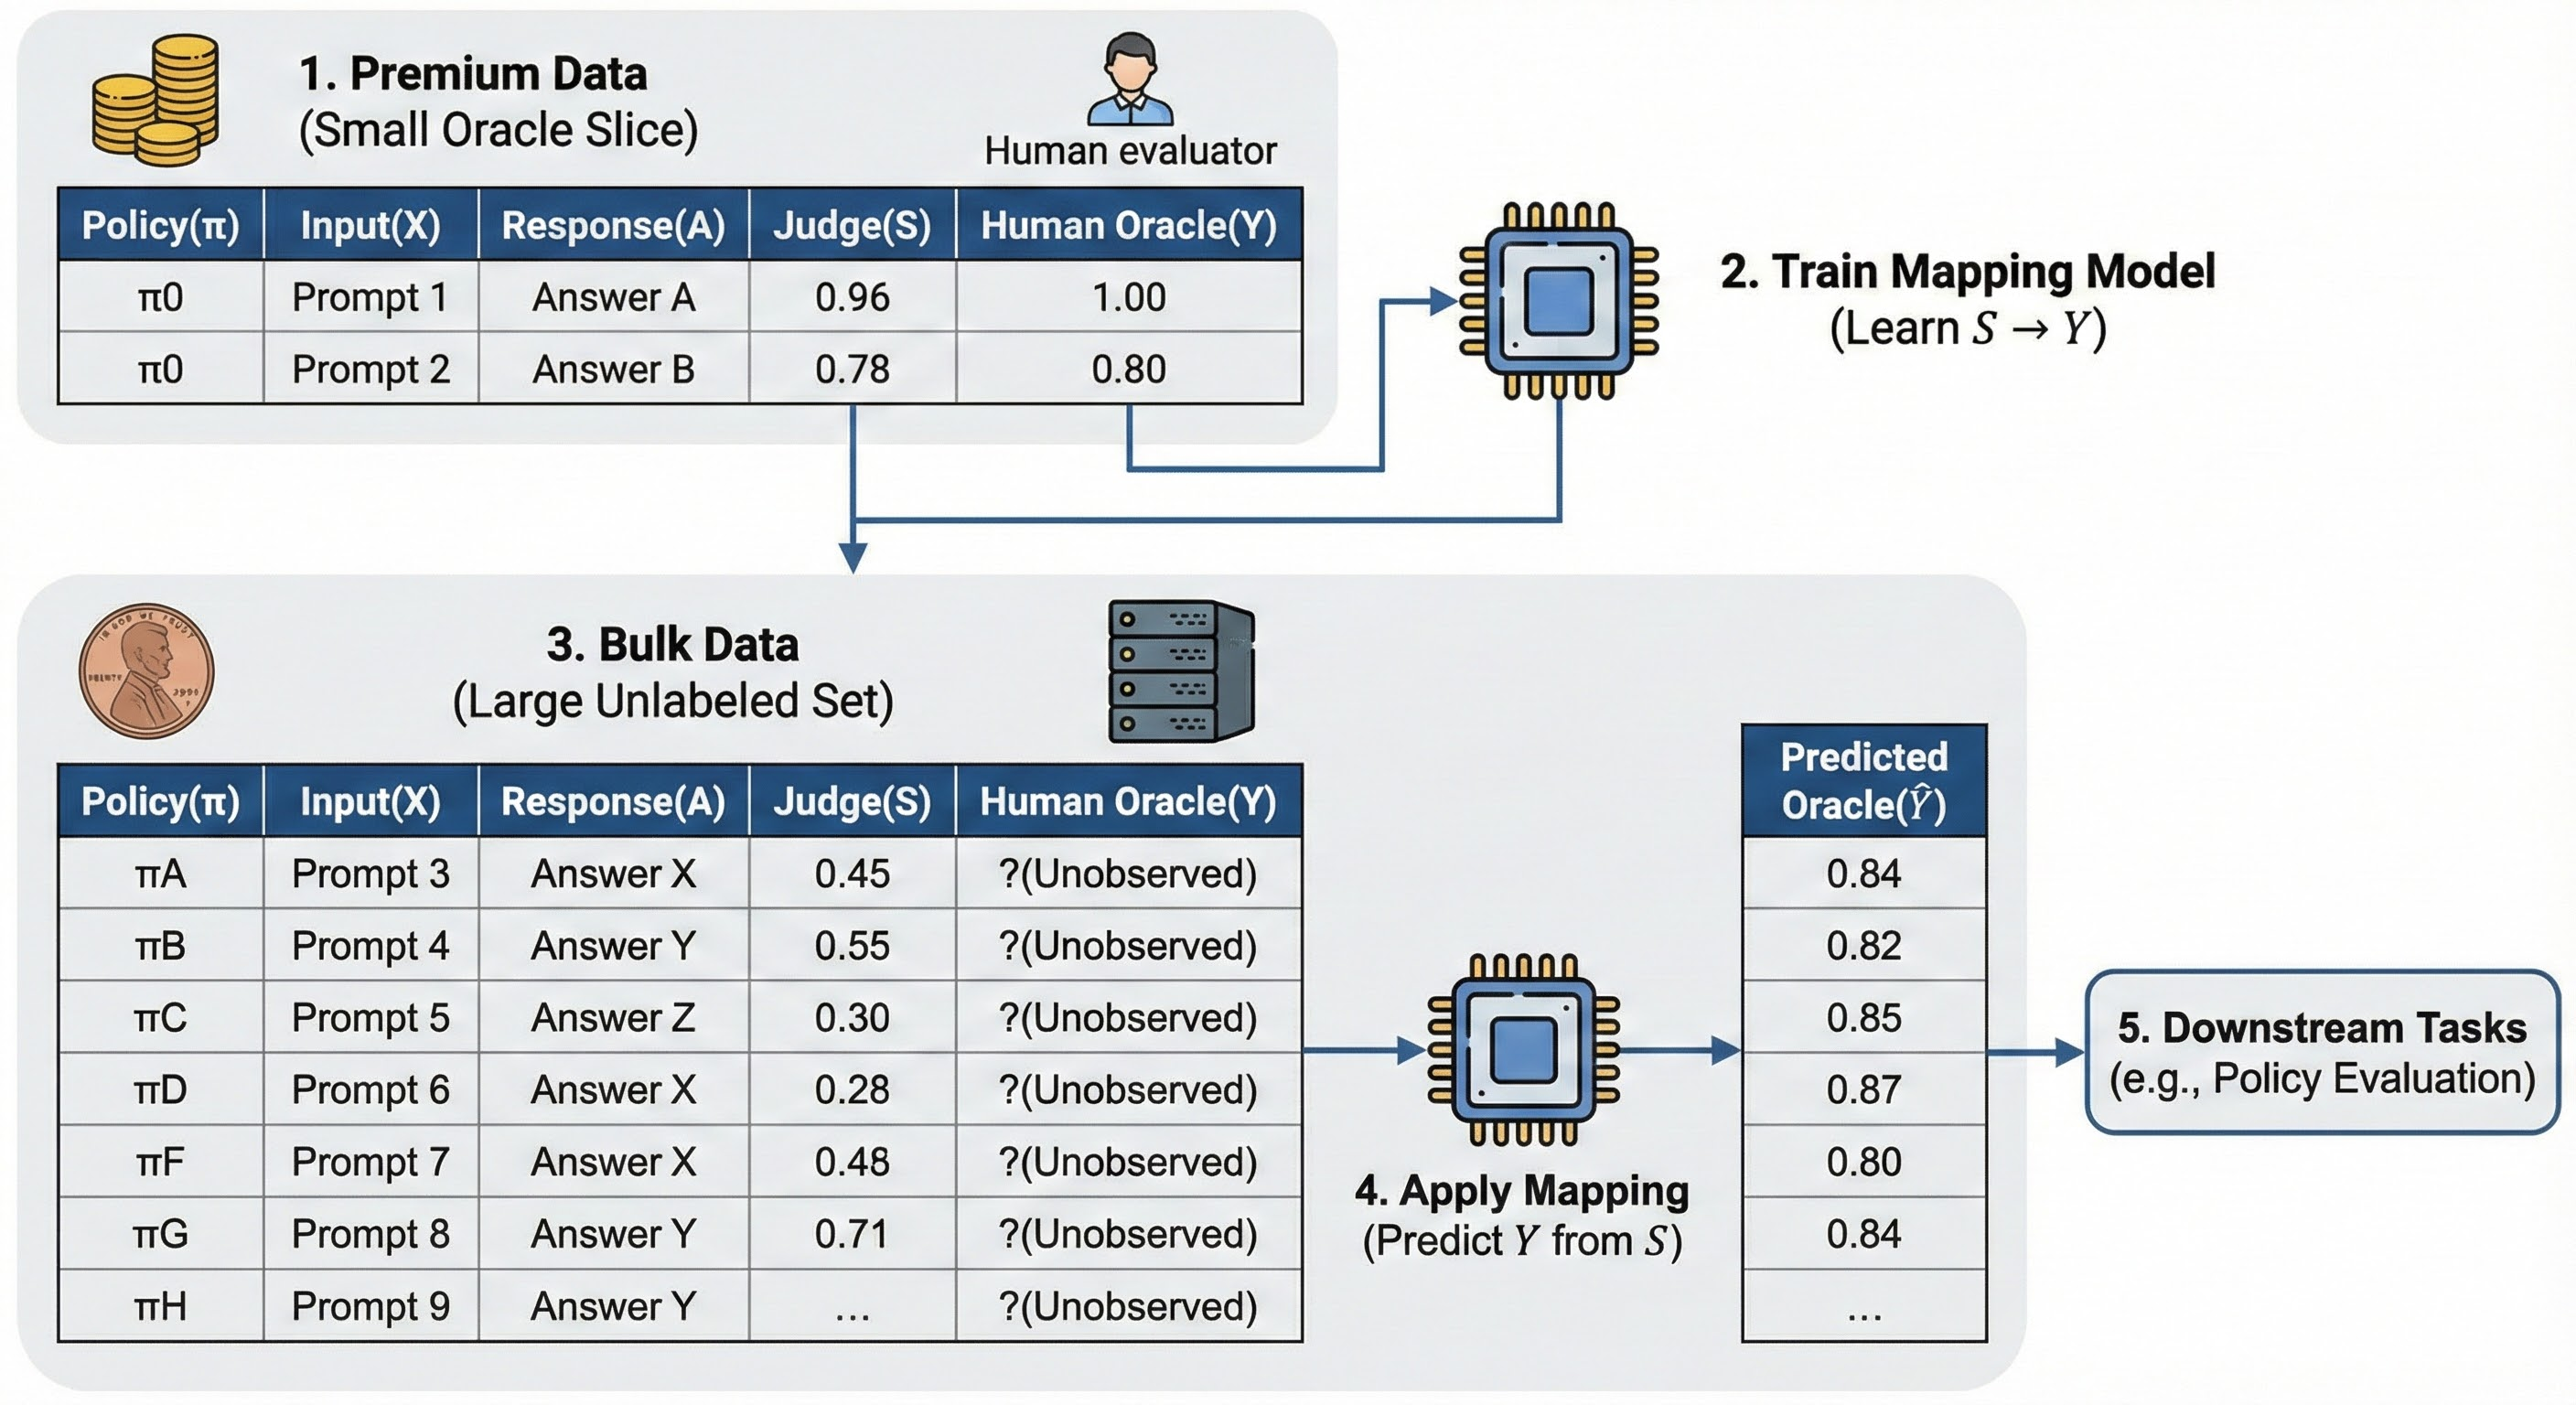
\includegraphics[width=\columnwidth]{figs/pipeline_overview.jpg}
  \caption{\textbf{CJE pipeline overview.} A small oracle slice (5--25\%) provides expensive oracle labels to train a calibration model ($S \to Y$). The learned mapping is then applied to bulk evaluation data where oracle labels are unavailable, enabling policy evaluation at a fraction of the cost. (In experiments, the oracle is \texttt{gpt-5-2025-08-07}; in production this would typically be human raters or downstream KPIs.)}
  \label{fig:pipeline}
\end{figure}

\CJE\ encodes justified knowledge as model restrictions: (i) monotonicity and mean-preservation for reward calibration, (ii) mean-one constraint with $S$-monotonicity for weights, (iii) nuisance-orthogonality for estimators, and (iv) convex combination for stacking. All learners are \emph{cross-fitted}; by the \emph{Efficiency via Model Restriction} theorem, these restrictions lower the efficiency bound (see \cref{sec:theory}).

\subsection{Reward calibration (two-stage isotonic)}
\label{ssec:method-autocal}
On the oracle slice $\{(S_i,Y_i)\}$, fit a \emph{mean-preserving} calibrator $R=f(Z(S))$ with $K$-fold
cross-fitting:
\begin{itemize}[leftmargin=*,itemsep=2pt,topsep=2pt]
\item Two-stage mode (recommended): Fit a smooth index $Z(S,X)=g(S,X)$
(splines+ridge), map to mid-ranks $U=\mathrm{ECDF}\{Z(S,X)\}$, then fit isotonic
$\hat h_{\uparrow}(U)$. Predictions are $R=\hat h_{\uparrow}(\mathrm{ECDF}\{g(S,X)\})$.
\item Monotone-only mode: Isotonic regression directly on $S$:
$\hat f_{\uparrow}\in\arg\min_{f\in\mathcal{M}_\uparrow}\sum_{i\in O}\big(Y_i-f(S_i)\big)^2$.
PAVA preserves the slice mean exactly. Use when covariates $X$ are unavailable.
\end{itemize}
\emph{Remark (covariate flexibility).} The terminal isotonic step preserves mean-honesty regardless of the first-stage model, so $g$ can be \emph{any} cross-fitted learner (splines, random forests, gradient boosting) and can incorporate covariates $X$ beyond $S$. In our experiments, including response length as a first-stage covariate improves ranking accuracy: LLM judges often favor longer responses independent of quality, and conditioning on length removes this confounder from the $S \to Y$ mapping.
Let $R^{\mathrm{OOF}}$ denote OOF predictions used along the IF path; the point
estimate may use the pooled fit. The terminal isotonic step makes the calibrator \emph{mean-honest} in either
mode. We treat $\hat f$ as learned and propagate its uncertainty via calibration-aware inference (\cref{ssec:method-oua}).

\begin{figure}[t]
  \centering
  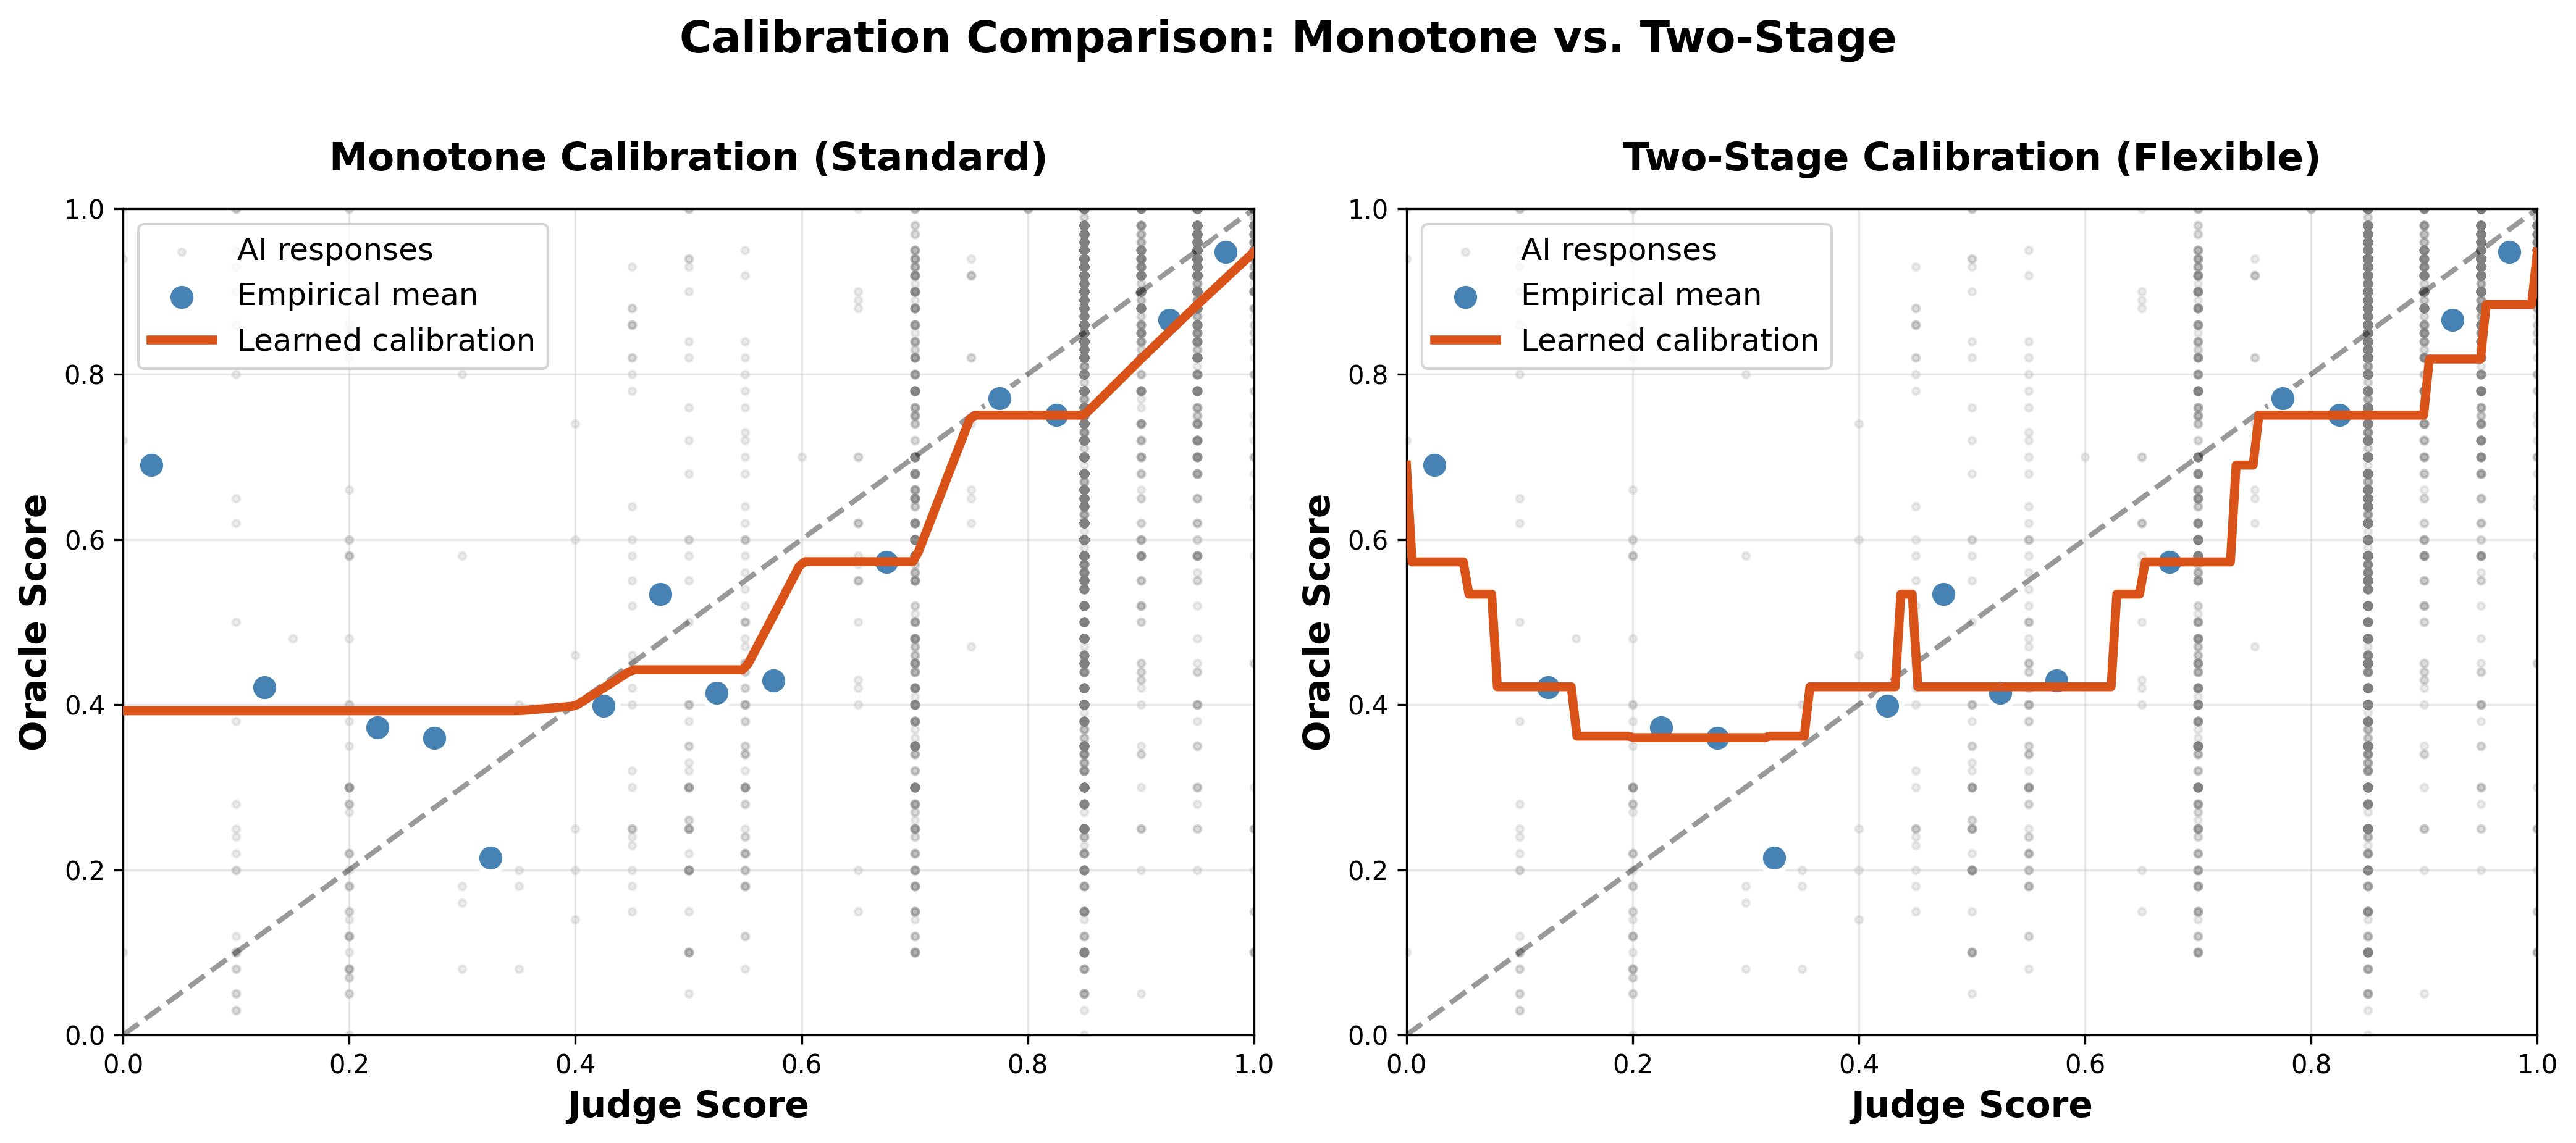
\includegraphics[width=\columnwidth]{figs/monotone_vs_two_stage.png}
  \caption{\textbf{Reward calibration: monotone vs.\ two-stage.} Left: monotone-only isotonic regression enforces monotonicity but cannot capture non-monotonic patterns in $\E[Y \mid S]$. Right: two-stage calibration (spline index $\to$ isotonic) can fit flexible patterns while preserving the mean.}
  \label{fig:reward-calibration}
\end{figure}

\subsection{Weight stabilization (unit-mean ratios via OOF stacking of $S$-monotone candidates)}
\label{ssec:method-simcal}
\emph{Scope and practical relevance:} Weight stabilization applies only to IPS and DR estimators. For open-ended generation under nontrivial policy shifts, coverage sparsity (low TTC) limits the utility of logged data (\cref{sec:intro}); in such regimes, Direct is preferred. Weight stabilization remains valuable in constrained settings (short outputs, near-clone shifts, tool-choice bandits) where TTC $\geq 0.70$, or when combining logged data with fresh draws via DR. The Direct method---which generates fresh responses under $\pi'$---requires no importance weights.

Let $W_{\pi'}^{\mathrm{m1}}$ be the self-normalized (SNIPS) baseline. For each fold $k$:
\begin{enumerate}[leftmargin=*,itemsep=2pt,topsep=2pt]
\item Monotone projections (train on $I_{\neg k}$): Fit increasing and decreasing isotonic maps on $S$
(the latter by running PAVA on $-S$), rescale each to mean one on $I_{\neg k}$, and predict OOF candidates on $I_k$:
$W_{\uparrow}^{\mathrm{OOF}}$, $W_{\downarrow}^{\mathrm{OOF}}$; optionally include an identity candidate
$W_{\mathrm{base}}^{\mathrm{OOF}}\equiv 1$.
\item OOF stacking (variance-aware): Define residuals $\Delta_i$ used by the downstream estimator:
$\Delta_i{=}R_i$ for IPS and $\Delta_i{=}R_i-\hat m(X_i,A_i)$ for DR (with $\hat m{=}\hat q$ below). Let
$U_c=W_c^{\mathrm{OOF}}\Delta$ for $c\in\{\mathrm{base},\uparrow,\downarrow\}$ and compute
$\hat\Sigma_{cd}=\mathrm{cov}(U_c,U_d)$ (tiny ridge if needed). Choose simplex weights
\[
\hat\beta\in\arg\min_{\beta\in\Delta_3}\ \beta^\top\hat\Sigma\,\beta,\qquad
W^{\mathrm{stack}}=\sum_c \hat\beta_c\,W_c^{\mathrm{OOF}},
\]
then renormalize $W^{\mathrm{stack}}$ to mean one.
\item Light variance guard (optional; $\rho{=}1$ by default): Cap variance at absolute threshold $\rho$:
\[
\alpha=\min\!\Big\{1,\ \sqrt{\frac{\rho}{\Var(W^{\mathrm{stack}})}}\Big\},\quad
W^{\mathrm{blend}}=1+\alpha\,(W^{\mathrm{stack}}-1),\quad
\hat W_{\pi'}=W^{\mathrm{blend}}/\bar W^{\mathrm{blend}}.
\]
Each step preserves (or restores) the sample mean. \emph{Note:} The theoretical guarantee (Lemma~\ref{lem:guard}) uses a \emph{relative} bound $\Var(\hat W)\le\rho\,\Var(W^{\mathrm{m1}})$; the implementation's absolute cap is more conservative when $\Var(W^{\mathrm{m1}}){>}1$.
\end{enumerate}
\emph{Remark (transport view).} In the continuous case the ideal component is
$m^\star(s)=p_{S\mid\pi'}(s)/p_{S\mid\pi_0}(s)$; weight stabilization stacks increasing and decreasing $S$-monotone candidates to minimize IF variance, yielding approximately monotone weights when one direction dominates.
When $m^\star(S)$ is not approximately monotone, isotonic projection trades bias for variance; in the low-overlap regimes where this matters most, we recommend Direct over IPS/DR (see CLE bound, \cref{sec:background}).
(Weight stabilization visualization in \cref{app:weight-viz}.)

\subsection{Estimators: Direct, Calibrated IPS, and Calibrated DR}
\label{ssec:method-estimators}
Let $\hat q(z)\approx \E[R\mid Z{=}z]$ be the cross-fitted calibrator (in experiments, $\hat q = \hat f^{(-k)}(Z)$; we do not fit a separate text-conditioned reward model).
Define $\hat g_{\pi'}(x)=\E_{\pi'}[\hat q(Z)\mid X{=}x]$; all nuisances are cross-fitted and OOF predictions
are used inside IFs.

\paragraph{Direct (fresh responses under $\pi'$; no overlap needed).}
When responses can be generated under the target policy, the Direct estimator uses calibrated rewards without importance weighting:
\[
\widehat V_{\mathrm{Direct}}(\pi') = \frac{1}{n}\sum_{i=1}^n R_i = \frac{1}{n}\sum_{i=1}^n \hat f(Z_i).
\]
For inference, the bias-corrected augmented estimator $\hat\theta_{\mathrm{aug}}$ (\cref{eq:theta-aug}) achieves ${\sim}$95\% coverage by correcting for calibration uncertainty.
Direct requires no overlap assumption and is the \textbf{recommended default} when fresh generation is feasible (\cref{tab:estimator-guide}).

\paragraph{Calibrated IPS.}
\[
\widehat V_{\mathrm{IPS}}(\pi')=\frac{1}{n}\sum_{i=1}^n \hat W_{\pi',i}\,R_i,\qquad
\phi^{\mathrm{IPS}}_i=\hat W_{\pi',i}\,R^{\mathrm{OOF}}_i-\widehat V_{\mathrm{IPS}}.
\]

\paragraph{Calibrated DR (doubly robust with calibrated rewards).}
\[
\widehat V_{\mathrm{DR}}(\pi')
=\frac{1}{n}\sum_{i=1}^n\Big\{\hat g_{\pi'}(X_i)+\hat W_{\pi',i}\big(R_i-\hat q(Z_i)\big)\Big\},
\quad
\phi^{\mathrm{DR}}_i=\hat g_{\pi'}(X_i)+\hat W_{\pi',i}\big(R^{\mathrm{OOF}}_i-\hat q^{\mathrm{OOF}}_i\big)-\widehat V_{\mathrm{DR}}.
\]

\emph{Remark (DR vs Direct).} DR combines an outcome model with a weighted residual correction. Under good overlap, the IPS component can improve efficiency; under poor overlap (TTC $< 0.7$), it adds noise. In our experiments, DR effectively reduces to its outcome model, and Direct achieves the same accuracy without requiring logprobs (\cref{sec:experiments}, Q3).

\subsection{Influence-function stacking (variance-optimal convex ensembling)}
\label{ssec:method-stack}
For a small library $\mathcal{E}$ of regular estimators (e.g., DR/TMLE/MRDR variants, capped IPS), form
the matrix of centered IF columns $\Phi=[\phi^{(e)}]_{e\in\mathcal{E}}$ (computed OOF on the same folds),
estimate $\hat\Sigma=\tfrac{1}{n}\Phi^\top\Phi+\lambda I$, and solve the simplex QP
\[
\hat\alpha\in\arg\min_{\alpha\in\Delta}\ \alpha^\top \hat\Sigma\,\alpha,\qquad
\widehat V_{\mathrm{stack}}=\sum_{e\in\mathcal{E}}\hat\alpha_e\,\widehat V^{(e)},\quad
\phi^{\mathrm{stack}}=\sum_{e\in\mathcal{E}} \hat\alpha_e\,\phi^{(e)}.
\]

\subsection{Calibration-aware inference}
\label{ssec:method-oua}

Standard CIs treat the calibration function $\hat f$ as fixed, ignoring first-stage estimation error. When the oracle slice is small, this understates total variance and produces severely narrow intervals. In our experiments, naive CIs on uncalibrated scores achieve 0\% coverage; bootstrap inference with bias-corrected estimation achieves ${\sim}$95\% coverage for Direct mode.

\paragraph{Variance decomposition.}
Total variance decomposes into two components:
\[
\Var_{\text{total}}(\widehat V) = \Var_{\text{eval}}(\widehat V \mid \hat f) + \Var_{\text{cal}}(\hat f),
\]
where $\Var_{\text{eval}}$ is the standard evaluation variance (estimated via the IF) and $\Var_{\text{cal}}$ is the variance due to calibration uncertainty.

\paragraph{Delete-one-fold jackknife.}
We estimate $\Var_{\text{cal}}$ via a delete-one-oracle-fold jackknife:
\begin{enumerate}[leftmargin=*,itemsep=2pt,topsep=2pt]
\item Partition the oracle slice into $K$ folds.
\item For each fold $k \in \{1,\ldots,K\}$, refit calibration omitting fold $k$: $\hat f^{(-k)}$.
\item Compute the leave-one-fold-out estimate: $\widehat V^{(-k)} = \widehat V(\hat f^{(-k)})$.
\item Estimate calibration variance:
\[
\widehat{\Var}_{\text{cal}} = \frac{K-1}{K} \sum_{k=1}^K \big(\widehat V^{(-k)} - \bar V\big)^2, \quad \bar V = \frac{1}{K}\sum_k \widehat V^{(-k)}.
\]
\end{enumerate}

\paragraph{Calibration-aware confidence intervals.}
\[
\widehat{\Var}_{\text{total}} = \widehat{\Var}_{\text{eval}} + \widehat{\Var}_{\text{cal}}, \qquad
\text{CI}_{95\%} = \widehat V \pm 1.96 \sqrt{\widehat{\Var}_{\text{total}}}.
\]
The calibration uncertainty share $\widehat{\Var}_{\text{cal}} / \widehat{\Var}_{\text{total}}$ ranges from 0\% (100\% oracle fraction, where no calibration is needed) to over 50\% (5\% oracle fraction), explaining why ignoring it produces catastrophically narrow CIs.

\paragraph{Bootstrap with bias-corrected estimation.}
While the jackknife captures variance, it does not correct for bias in the plug-in estimator $\widehat V = n^{-1}\sum_i \hat f(S_i)$. This bias arises because $\hat f$ is fit on the oracle slice and applied to all samples, creating a covariance between the calibration function and the evaluation samples. We address this with the one-step estimator derived from the efficient influence function for missing-outcome estimation (\cref{app:eif-direct}; see also \citet{Chen2026EfficientLLMJudge} for the LLM-as-judge instantiation):
\begin{equation}
\label{eq:theta-aug}
\hat\theta_{\mathrm{aug}} = \frac{1}{n}\sum_{i=1}^n \hat f(S_i) + \frac{1}{|L|}\sum_{i \in L}\big(Y_i - \hat f^{(-i)}(S_i)\big),
\end{equation}
where $\hat f$ is the full calibrator, $\hat f^{(-i)}$ is the calibrator trained on folds excluding sample $i$'s cluster, and $L$ is the oracle slice. The first term uses the full calibrator for lower variance; the second term uses cluster-out-of-fold predictions to avoid overfitting in the residual correction. If oracle sampling is non-uniform (e.g., oversampling uncertain prompts), replace the constant $|L|/n$ with sample-specific inclusion probabilities $e(Z_i)$ in the general AIPW form (\cref{app:eif-direct}). Combined with bootstrap (refitting the calibrator in each replicate), this achieves ${\sim}$95\% coverage across oracle fractions (\cref{tab:uq-comparison}), compared to 70--89\% for jackknife-only variance estimation.

\paragraph{Computational cost.}
Bootstrap with $\hat\theta_{\mathrm{aug}}$ requires $B$ refits of the reward calibrator (we use $B{=}2{,}000$). Since isotonic regression is $O(n \log n)$, the overhead remains modest relative to the cost of teacher forcing and response generation. The full bootstrap procedure (\cref{alg:bootstrap-direct}) uses prompt-level cluster resampling to preserve within-prompt dependence \citep{CameronGelbachMiller2008}, with a resample-until-valid loop ensuring each replicate has sufficient oracle labels.